\section{Metode}
\noindent\textbf{Utstyr}:
\begin{itemize}
    \item Telefon
    \item Telefonholder
    \item Trefot
    \item Vater
\end{itemize}

\begin{figure}
    \centering
    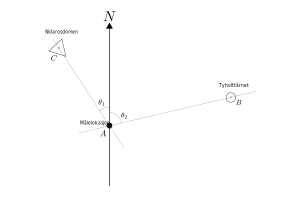
\includegraphics[width=\textwidth]{img/angle_north.pdf}
    \caption{Koordinatene til $B$ og $C$ blir estimert ved hjelp av Google Maps. 
    Koordinatene til målelokasjonen $A$ ble målt ved hjelp av Phyphox.
    $\theta_1$ og $\theta_2$ er hhv. vinkel mellom spiret på Nidarosdomen og nord, og mellom Tyholttårnet og nord. 
    Disse regnes ut ved å finne lengden til linjestykkene $\overline{AP_1}, \overline{BP_1}$ og $\overline{AP_2}, \overline{CP_2}$}.
    \label{fig:angle_north}
\end{figure}

For å finne vinkelen mellom referansepunktet og nord ser man på den rettvinklede trekanten med hjørner i målelokasjon, referansepunktet og et tredje punkt med samme lengdegrad som målelokasjonen og samme breddegrad som referansepunktet.
Tangens til $\theta$ er gitt ved $\overline{CP_2} / \overline{AP_2}$.
For å få riktig fortegn på vinkelen multipliseres det med $\text{sgn}(A_{\text{breddegrad}} - C_{\text{breddegrad}})$. Positiv vinkel blir da mot klokken sett ovenfra.
\par
For å regne ut avstandene ble python-biblioteket \textit{GeoPy} (\ref{geopy}) brukt.

